\documentclass[tikz,border=12pt]{standalone}
\usepackage{tikz}
\usetikzlibrary{calc}

\begin{document}
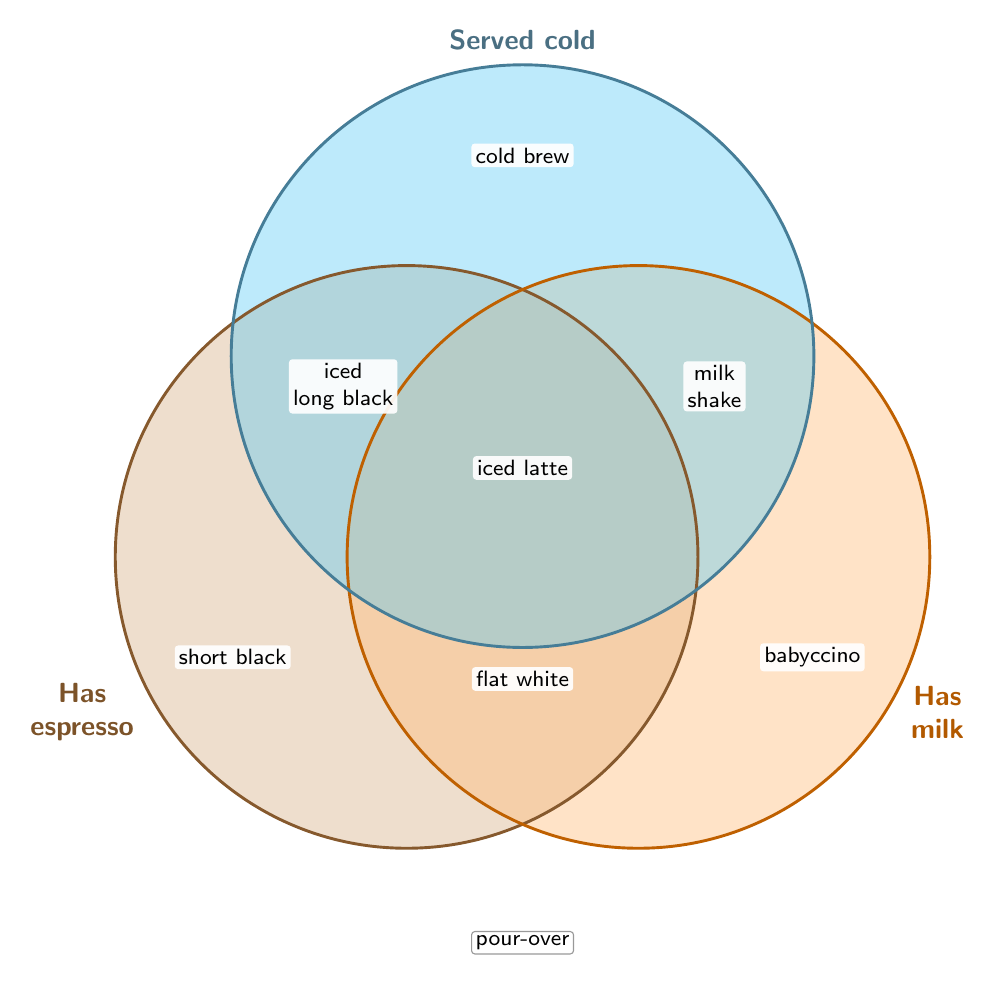
\begin{tikzpicture}[
  font=\sffamily,
  drink/.style={
    align=center,
    font=\sffamily\footnotesize,
    inner sep=1.5pt,
    fill=white,
    fill opacity=0.92,
    text opacity=1,
    rounded corners=1.2pt
  },
  setlabel/.style={
    align=center,
    font=\sffamily\bfseries,
    inner sep=1pt
  }
]

  % Equal circles whose centres form an equilateral triangle.
  \coordinate (E) at (210:1.7); % Has espresso
  \coordinate (M) at (330:1.7); % Has milk
  \coordinate (C) at (90:1.7);  % Served cold
  \def\R{3.7}

  \fill[brown!62,  opacity=0.42] (E) circle (\R);
  \fill[orange!55, opacity=0.40] (M) circle (\R);
  \fill[cyan!65,   opacity=0.40] (C) circle (\R);

  \draw[brown!70!black,  line width=1.05pt] (E) circle (\R);
  \draw[orange!75!black, line width=1.05pt] (M) circle (\R);
  \draw[cyan!55!black,   line width=1.05pt] (C) circle (\R);

  % Set names, just outside each circle.
  \node[setlabel, text=brown!65!black,  anchor=east]  at (210:5.65) {Has\\espresso};
  \node[setlabel, text=orange!70!black, anchor=west]  at (330:5.65) {Has\\milk};
  \node[setlabel, text=cyan!45!black,   anchor=south] at (90:5.55)  {Served cold};

  % Exclusive crescents.
  \node[drink] at ($(E)+(210:2.55)$) {short black};
  \node[drink] at ($(M)+(330:2.55)$) {babyccino};
  \node[drink] at ($(C)+(90:2.55)$)  {cold brew};

  % Pairwise lenses. Labels are small and sit on each lens midline,
  % outside the third circle.
  \node[drink] at ($(E)!0.5!(C)+(150:1.78)$) {iced\\long black};
  \node[drink] at ($(M)!0.5!(C)+(30:1.78)+(0.16,0)$) {milk\\shake};
  \node[drink] at ($(E)!0.5!(M)+(270:1.55)$) {flat white};

  % All three sets.
  \node[drink] at (0,0.28) {iced latte};

  % None of the three.
  \node[drink, draw=black!40] at (0,-5.75) {pour-over};

\end{tikzpicture}
\end{document}
